\documentclass{article}

\usepackage[algoruled]{algorithm2e}
\usepackage{amsmath}
\usepackage{amssymb}
\usepackage{caption}
\usepackage{color}
\usepackage{dsfont}
\usepackage{float}
\usepackage{graphicx}
\usepackage{sidecap}
\usepackage{subcaption}
\usepackage{url}
\usepackage{wrapfig}

\newcommand{\hilight}[1]{\colorbox{yellow}{#1}}

\title{Course Project for CSE 6740 / CS 7641 Summer 2012
  : EM for Sparse and Non-Negative PCA}
\author{Nobles, Mallory \\ \texttt{mallory.nobles@gmail.com}
  \and Martin, Christopher \\ \texttt{chris.martin@gatech.edu}
  \and Rice, Emily \\ \texttt{ricemily84@gmail.com} }
\date{}

\begin{document}
\maketitle

In their paper, ``Expectation-Maximization for Sparse and Non-Negative PCA'',
Sigg and Buhmann develop an algorithm for finding principle components where
there are two additional constraints on these vectors:
a cardinality constraint and a non-negativity constraint.
The cardinality constraint ensures that there are a limited number
of non-zero elements in the principle components, while
the non-negativity constraint guarantees that no elements of
the principle components are negative.

Both of these constraints have practical importance and facilitate
interpretability and applicability.
Typically in PCA, the dominant eigenvectors are difficult to interpret
because they are linear combinations of all of the observed variables,
and these linear combinations ``may mix both positive and negative weights,
which might partly cancel each other'' (Zass 2006).
Sparse, non-negative PCA addresses both of these issues.
Futhermore, the restrictions that these constraints impose on the
principle components are natural in many applications of PCA.
For example, in finance, sparse factors mean that there are
fewer assets in the portfolio, which implies lower transaction costs.

While it is desirable to be able to impose these constraints on
the problem of estimating principle components, doing so has
computational challenges. If either sparsity or non-negativity
is enforced, the problem of determining the first principle component
(finding the solution to \[
\arg\max_{\mathbf{w}} \mathbf{w}^\intercal C\mathbf{w}
\textrm{ s.t. } \|\mathbf{w}\|_2 = 1
\]
where $C$ is the covariance matrix of the sample data) is NP-hard.
Others have developed algorithms that test global optimality, although
the computation time is $O(D^3)$ where $D$ is the dimension of the data.

In this paper, Sigg and Buhmann claim to develop an $O(D^2)$ algorithm
that enforces either the cardinality constraint,
the non-negativity constraint, or both.
Given the reduction in complexity, they note that this algorithm is
especially useful for high-dimensional data (where $D >> N$).
Other supposed advantages of the algorithm are that it is possible
to specify the desired cardinality $K$ directly, which is not possible
in much of the previous work, and the algorithm does not require
direct work on the covariance matrix $C$, which is costly to obtain
when $D$ or $N$ are large.

\section{Theory}

Sigg and Buhmann use an EM (expectation-maximization) algorithm
to compute the first principle component at a given sparsity.
They then build upon this algorithm to find the first non-negative
principle component at a given sparsity and compute additional
principle components.

To develop their main algorithm for computing a sparse first principle
component, they begin by noting that the $\mathbf{w}_{t+1}$
specified by the M-step in an EM algorithm is the same vector as the
solution for the quadratic program
$\displaystyle\mathbf{w}^* = \arg\min_{\mathbf{w}} J(\mathbf{w})$
where $J(\mathbf{w}) = h \mathbf{w}^\intercal \mathbf{w}
  - 2 f^\intercal \mathbf{w}$,
$h = \sum_{n=1}^N y_n^2$,
$f = \sum_{n=1}^N y_n \mathbf{x}_{(n)}$,
and $y = \mathbf{x} \mathbf{w}_{(t)}$.

~

\begin{wrapfigure}{r}{0.5\textwidth}
\caption{Gradient descent step}
\label{fig:gd}
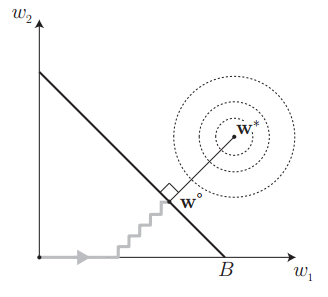
\includegraphics[width=0.5\textwidth]{gd.png}
\end{wrapfigure}

The authors then call upon the fact that enforcing a constraint
on $\|\mathbf{w}\|_1$ favors a sparse solution.
To solve the modified problem
\[
\mathbf{w}^\circ = \arg\min_{
  \mathbf
{w} : \|\mathbf
{w}\|_1 \le B
} J(\mathbf{w})
\]
they use an axis aligned gradient descent procedure
described on 4 of their paper (and their illustration
is reprinted here in Figure \ref{fig:gd}).
When incorporating a non-negative constraint, they claim that it is
optimal to set $w_i = 0$ for all $i$ such that $f_i < 0$
and solve for the other elements of $\mathbf{w}$ as in the above process.

Finally, Sigg and Buhmann argue that it is optimal to initialize
the sparse PCA algorithm with the first unconstrained principle component
and to initialize the non-negative PCA algorithm with a random unit vector
in the non-negative orthant.
They claim that when this vector is the input to their sparse algorithm,
the algorithm finds the global optimum.
This is not the case for the non-negative, sparse algorithm.

The authors explain how finding the first principle component
$\mathbf{w}_{(1)}$ leads directly to an iterative algorithm
for finding the others.
This is accomplished by calculating $\mathbf{X} P$
where \[ P = I - \mathbf{w}_{(1)} \mathbf{w}_{(1)}^\intercal \textrm{.} \]
$\mathbf{X}P$ is the projection of the data onto the subspace orthogonal
to the first principle component.
The first principle component of $\mathbf{X} P$ is the second
principle component of $\mathbf{X}$, so re-running the algorithm
on subsequent projections yields additional principle components.

\section{Implementation}

To implement Sigg and Buchmann's algorithm for sparse PCA,
we use Algorithm \ref{alg:sparse}, which is detailed on
page 5 of their paper.

\begin{algorithm}[h]\dontprintsemicolon
  \caption{EM for Sparse PCA}
  \label{alg:sparse}
  \KwData{
    $\mathbf{X} \in \mathds{R}^{N \times D}$,
    $K \in [1,D]$,
    $\varepsilon$
  }
  \KwResult{
    The first principle component of $\mathbf{X}$
    having cardinality $K$.
  }
  $t \leftarrow 1$ \;
  $\mathbf{w_{(t)}} \leftarrow$ first principle component
  of unconstrained PCA on $\mathbf{X}$ \;
  \Repeat{$| \mathbf{w}_{(t+1)}^\intercal \mathbf{w}_{(t)} |
      > 1 - \varepsilon$}{
    $\mathbf{y} \leftarrow \mathbf{X} \mathbf{w}_{(t)}$ \;
    $\mathbf{w^*} \leftarrow f / h$ \;
    $\mathbf{s} \leftarrow$ elements of $|w_i^*|$
      sorted in descending order \;
    $\boldsymbol\pi_1 \leftarrow$ indices of sorting order \;
    $\boldsymbol\pi_2 \leftarrow$ indices of sorting order
      when $\boldsymbol\pi_1$ is sorted in ascending order \;
    $\mathbf{w}_{(t+1)} \leftarrow 0$ \;
    \For{$k = 1 \ldots K$} {
      Add $(\mathbf{s}_k - \mathbf{s}_{k+1})$
      to elements $1,\ldots,k$ of $\mathbf{w}_{(t+1)}$
    }
    $\mathbf{w}_{(t+1)} \leftarrow \mathbf{w}_{(t+1)}$
      permuted according to $\boldsymbol\pi_2$ \;
    $\mathbf{w}_{(t+1)} \leftarrow \mathbf{w}_{(t+1)}$ $\circ$
      sign$(\mathbf{w^*}) / \|\mathbf{w}_{(t+1)}\|_2$ \;
    $t \leftarrow t + 1$
  }
  \Return $\mathbf{w}$
\end{algorithm}

Note that we compute the first principle component of the
unconstrained problem using another procedure described by
page 3 of Sigg and Buhmann's paper.
We choose sufficiently small $\varepsilon$ so that repeated
iterations of the algorithm yield consistent estimates of
the first principle component.

To implement non-negative sparse PCA, we used Algorithm \ref{alg:nonneg}.
As in Algorithm \ref{alg:sparse},
$\mathbf{X} \in \mathds{R}^{ N\times D}$ and $K \in \{1, \ldots, D\}$.
This algorithm calls heavily upon the underlying algorithm for
estimating sparse principle components.
Note that since this algorithm may find local optima,
for each cardinality K we run the algorithm ten times
and select the most successful implementation.
Because this non-negative algorithm is not discussed in great depth
in the paper, to determine this procedure, we consulted the code
provided by the author at
\url{http://www-oldurls.inf.ethz.ch/personal/chrsigg/icml2008/}.

\begin{algorithm}[h]\dontprintsemicolon
  \caption{Non-Negative Sparse PCA}
  \label{alg:nonneg}
  \KwData{
    $\mathbf{X} \in \mathds{R}^{N \times D}$,
    $K \in [1,D]$,
    $\varepsilon$
  }
  \KwResult{
    The first non-negative sparse principle component of $\mathbf{X}$
    having cardinality $K$.
  }
  \For{$i \in [1,10]$} {
    $t \leftarrow 1$ \;
    $\mathbf{w_{(t)}} \leftarrow$
      random unit vector in non-negative orthant \;
    \Repeat{$| \mathbf{w}_{(t+1)}^\intercal \mathbf{w}_{(t)} |
        > 1 - \varepsilon$}{
      $\mathbf{y} \leftarrow \mathbf{X} \mathbf{w}_{(t)}$ \;
      $f^{\textrm{index}} \leftarrow i : f_i > 0$ \;
      $f \leftarrow f[f^{\textrm{index}}]$ \;
      $\mathbf{w^*} \leftarrow f / h$ \;
      $\mathbf{s} \leftarrow$ elements of $|w_i^*|$
        sorted in descending order \;
      $\boldsymbol\pi_1 \leftarrow$ indices of sorting order \;
      $\boldsymbol\pi_2 \leftarrow$ indices of sorting order
        when $\boldsymbol\pi_1$ is sorted in ascending order \;
      $\mathbf{w}_{(t+1)} \leftarrow 0$ \;
      $\mathbf{w^f}_{(t+1)} \leftarrow 0$ \;
      \For{$k = 1 \ldots K$} {
        Add $(\mathbf{s}_k - \mathbf{s}_{k+1})$
        to elements $1,\ldots,k$ of $\mathbf{w^f}_{(t+1)}$
      }
      $\mathbf{w^f}_{(t+1)} \leftarrow \mathbf{w^f}_{(t+1)}$
        permuted according to $\boldsymbol\pi_2$ \;
      $\mathbf{w^f}_{(t+1)} \leftarrow \mathbf{w^f}_{(t+1)}$ $\circ$
        sign$(\mathbf{w^*}) / \|\mathbf{w^f}_{(t+1)}\|_2$ \;
      $\mathbf{w}_{(t+1)}[f^{\textrm{index}}] \leftarrow
        \mathbf{w^f}_{(t+1)}$\;
      $t \leftarrow t + 1$
    }
  }
  \Return The $\mathbf{w}$ that maximizes $\textrm{var}(\mathbf{Xw})$
\end{algorithm}

\section{Experiments}

Through their experiments, the authors explore how their algorithms perform
when the data has dimensions $N \times D$ such that $D < N$ and $D >> N$.
To consider the case when $D < N$, they use a $2429 \times 361$ data set
of CBCL face images.
To consider the case when $D >> N$, they use a $72 \times 12582$ data set
describing the gene sequences of leukemia patients.

For both data sets, the authors show how the variance explained by the first
principle component changes as the cardinality of the component varies.
They compare these results to those of other popular sparse PCA algorithms.
For the gene data, they also show the time needed to compute a sparse
first principle component using the various algorithms.

Similarly, for the face image data, the authors show how the variance
explained by the first, non-negative principle component varies given
its cardinality.
They compare this to results from another non-negative, sparse PCA algorithm.
Furthermore, they show that the cumulative variance increases as additional
non-negative, sparse principle components are considered.
They repeat this experiment for two cases. In the first case they enforce
the requirement that principle components be orthogonal, and in the second
they allow quasi-orthogonal components.

Finally, Sigg and Buhmann consider the usefulness of their algorithms
for classification.
They use their algorithms to perform feature selection on the gene data.
Then, they use $k$-means ($k=3$) to cluster the reduced data
and compare the clustering assignments to the true labels of the gene data,
which identify the patent's type of leukemia.
Here, the authors measure agreement using Jacard scores.
The Jacard score ``reflects the intersection over union between the
[k-means] clustering assignments and the expected classification''.
More specifically, $J = \cap_{11} / (\cap_{11} + \cap_{01} + \cap_{10})$
where $\cap_{11}$ is the number of pairs of instances that are
classified together in both the algorithm's assignments and the true labels,
$\cap_{01}$ is the number of pairs that are classified together by the
algorithm but do not share the same true label, and $\cap_{10}$ is the
number of pairs that share the same true label but are not classified
together by the algorithm.
Note that the range of $J$ is $[0, 1]$, where $0$ indicates no match
and $1$ indicates a perfect match.
The authors estimate the mean and standard deviation of $J$ when they
cluster using
between $1$ and $250$ features chosen with both sparse PCA and
sparse, non-negative PCA.

\begin{figure}[h,width=\textwidth]
\caption{Variance versus cardinality for gene data}
\label{fig:jacard}
\begin{subfigure}{0.5\textwidth}
\caption{Our results}
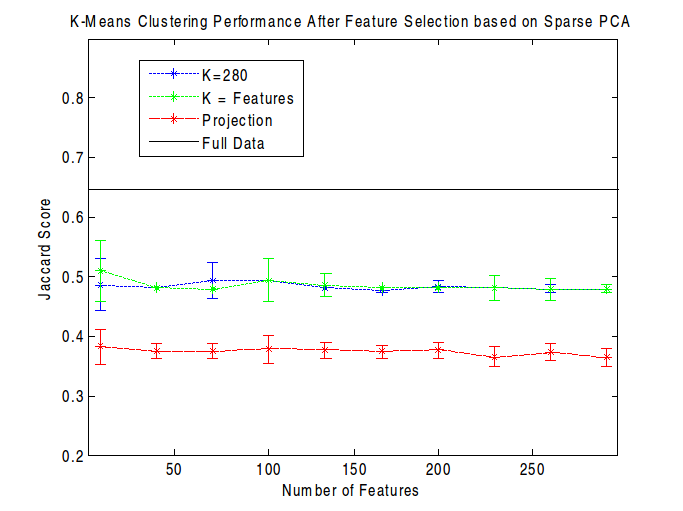
\includegraphics[width=\textwidth]{8.png}
\end{subfigure}
\begin{subfigure}{0.5\textwidth}
\caption{Their results}
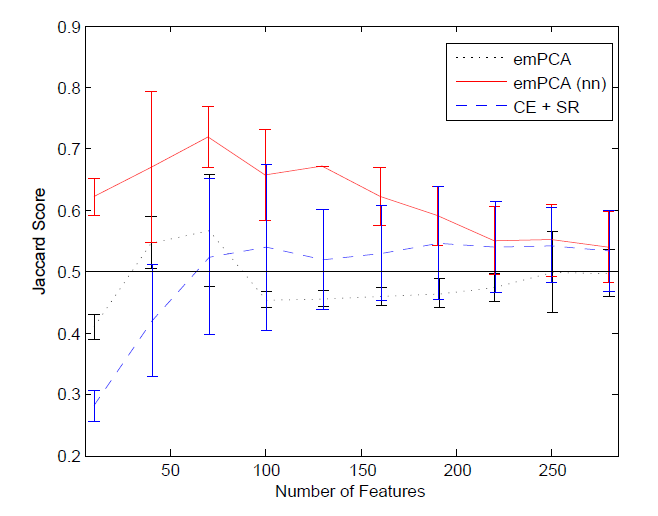
\includegraphics[width=\textwidth]{7.png}
\end{subfigure}
\end{figure}

\section{Results}

We were able to successfully replicate Sigg and Buhmann's graph of
cardinality versus variance explained by the first sparse
principle component for the gene data ($D >> N$).
Figure \ref{fig:gene-variance} compares these results.

\begin{figure}[h,width=\textwidth]
\caption{Variance versus cardinality for gene data}
\label{fig:gene-variance}
\begin{subfigure}{0.5\textwidth}
\caption{Our results}
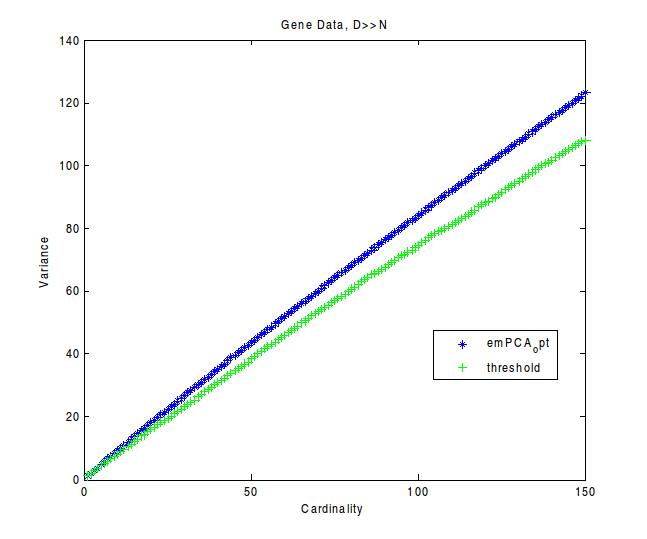
\includegraphics[width=\textwidth]{2.png}
\end{subfigure}
\begin{subfigure}{0.5\textwidth}
\caption{Their results}
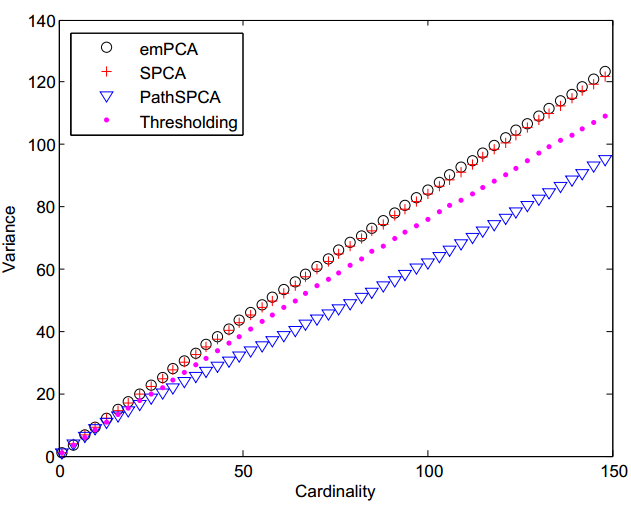
\includegraphics[width=\textwidth]{1.png}
\end{subfigure}
\end{figure}

Furthermore, we founds that the computation time of their sparse
PCA algorithm was very fast for the gene expression data.
However, we found that the other algorithms also performed well,
and we were not able to replicate the discrepancies between
running times claimed by Sigg and Buhmann.
This is shown in Figure \ref{fig:timing}.

\begin{figure}[h,width=\textwidth]
\caption{Running time versus cardinality}
\label{fig:timing}
\begin{subfigure}{0.5\textwidth}
\caption{Our results}
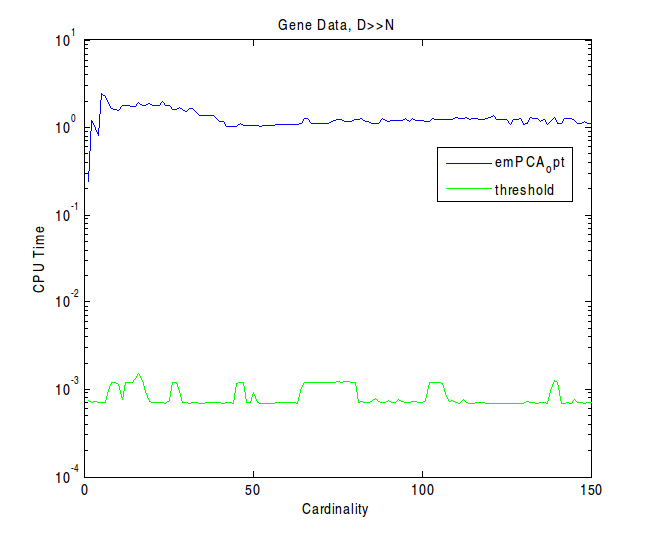
\includegraphics[width=\textwidth]{6.png}
\end{subfigure}
\begin{subfigure}{0.5\textwidth}
\caption{Their results}
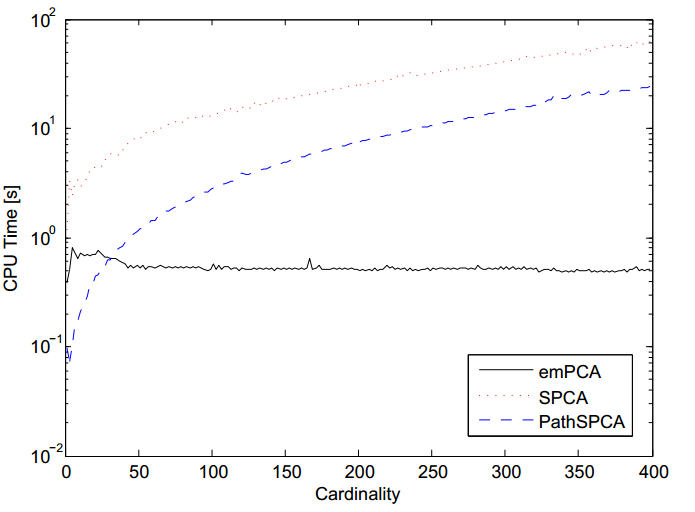
\includegraphics[width=\textwidth]{5.png}
\end{subfigure}
\end{figure}

We also had difficulty reproducing the variance results for the
face image data. Our results were of a generally similar character
as those reported by the paper authors, but we found that the variance
explained by the first principle component was significantly smaller
for each algorithm than the authors reported, as we show
in Figure \ref{fig:face-variance}.

\begin{figure}[h,width=\textwidth]
\caption{Variance versus cardinality for face data}
\label{fig:face-variance}
\begin{subfigure}{0.5\textwidth}
\caption{Our results}
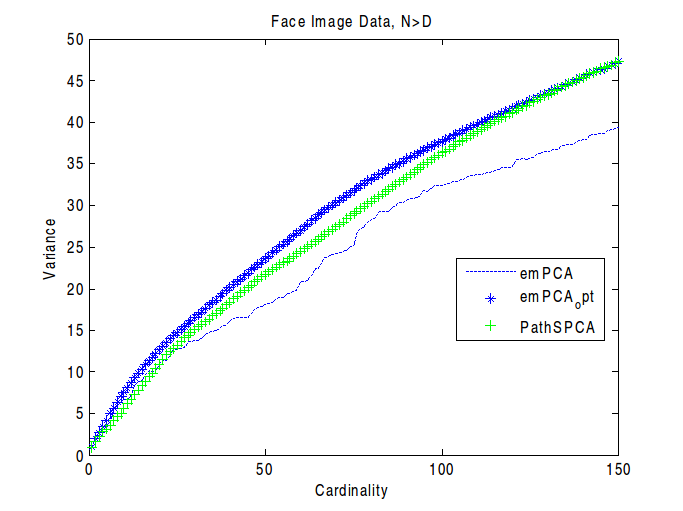
\includegraphics[width=\textwidth]{4.png}
\end{subfigure}
\begin{subfigure}{0.5\textwidth}
\caption{Their results}
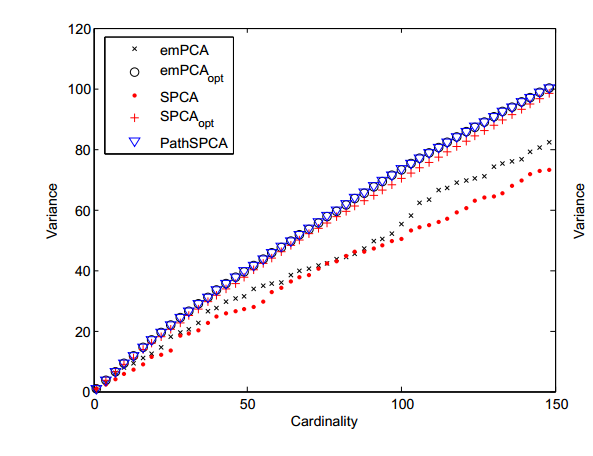
\includegraphics[width=\textwidth]{3.png}
\end{subfigure}
\end{figure}

Because the values of the variance are consistently deflated
across all algorithms, we suspect that the authors may have
applied some treatment to either the data or the results
that is not explicitly described in their paper.

When performing non-negative, sparse PCA on the face data,
we find that the variance explained by each non-negative
sparse first principle component is very similar to the
variance explained by the sparse first principle component
of the same cardinality.
As the authors note, this is because the first principle component
for the face data lies in the non-negative orthant, so this is the
trivial case of non-negative, sparse PCA.
To account for this, the authors project the data onto the orthogonal
subspace of the first principle component.
However, we do not make this correction because we feel that this
distorts the results, since this is the same step taken to compute
additional principle components.
We also noticed that the explained variance curve was less smooth
for the non-negative sparse PCA than for sparse PCA.
This is because sparse PCA is finding global optimizers, which
some iterations of non-negative sparse PCA find local optima.

Our attempts to compute multiple principle components were not successful.
We found that our computer did not have sufficient memory to perform the
projections necessary to compute multiple components for the gene data,
even when the code was run on the Condor server. Furthermore, while we
were able to compute multiple approximately orthonormal sparse principle
components, the cumulative variance explained curve was not concave.

Finally, we considered how sparse PCA could be used to enhance
classifications methods.
Sigg and Buhmann explain that they ``apply emPCA to select a
subset of genes of the leukemia data \ldots [and] for each gene subset,
we cluster the data using k-means ($k=3$) and compare the cluster
assignments to the true labeling of the data.''
However, they do not further indicate how they employ their
sparse PCA algorithm for feature selection.

Other authors have proposed various methods for feature selection
with sparse PCA.
To consider n features, some suggest computing a sparse principle
component and selecting the features that correspond to the $k$
largest values in the absolute value of the loadings vector.
Others suggest computing a sparse PC of cardinality $n$ and using
all features that correspond to non-zero elements of the loadings vector.
Finally, others propose performing classification on the principle
components, rather than on the data.
We find that the last method is the least successful when only one
principle component is considered.
The other two methods perform similarly, especially for large
numbers of features.

\section{Analysis}

One of Sigg and Buhmann's primary claims is that due to their
relatively low complexity, their algorithms are particularly
well suited to handle cases when $D$ is very large.
However, their experiments do not strongly support this claim.
In the figures that plot cardinality against variance
explained by the first principle component, we see that for the
gene data when $D >> N$, all of the algorithms perform very
similarly. There is actually a larger variation in performance
among algorithms for the face image data when $N$ is closer to $D$.
Furthermore, in both cases, while Sigg and Buhmann's algorithm
performs well compared to the other algorithms, its advantage is small.
We also do not find evidence of their algorithm improving run times
in this case.

Finally, given their argument that their algorithms offer a particular
advantage when $D >> N$, it is unclear to us why the authors choose
to focus on the face image data when reporting their results for
non-negative sparse PCA.

During our analysis, we also find evidence of potential disadvantages
of Sigg and Buhmann's algorithms that the authors do not address.
For example, while the run time of the sparse PCA algorithm was
very fast for the gene expression data, this did not hold true for
the face image data.
Since we believe that the authors may have applied some
treatment to the face data before running their algorithms,
we suspect that the performance of the algorithms may be
impacted by this change in the form of the data.

Long run times of the sparse PCA algorithm
became a problem when performing the non-negative sparse PCA algorithm
because each non-negative sparse PCA iteration includes
ten runs of an algorithm very similar to the sparse algorithm.

Finally, we feel that the authors focus too exclusively on
the first principle component.
In practical applications, the variance explained by the first
principle component is less important than the cumulative variance
captured the first several principle components.

\section{Extensions}

We feel that Sigg and Buhmann's paper could be strengthened
through several additional experiments. First,
D'Aspremont, El Ghaoul and Zhang
use an alternative procedure for assessing the success of
sparse PCA algorithms that we feel is more appropriate than
Sigg and Buhmann's plots of cardinality versus variance explained
by the first principle component.
In their method, D'Aspremont, El Ghaoul and Zhang
determine the cardinality needed for the
first sparse PC to explain 90\% of the variance explained
by the unconstrained, full first PC.
They then compute the first three principle components at this
cardinality and determine the cumulative variance explained by
these three components. They do this for each algorithm they
wish to compare. This procedure has several advantages.
First, it captures information about the cost in statistical
fidelity of sparsity and compares the performance of the sparse algorithm
to that of unconstrained PCA. It also gives a more complete
description of the performance of each sparse algorithm, which
facilitates comparison among them.

We also feel that the paper should include a description of
results for non-negative sparse PCA applied to the gene data,
since this is a more relevant data set to the problem of
efficient dimension reduction.

\end{document}
